\section[Continuity and spatial averaging in ion-acoustic reconnection diagnostics]{\raggedright Continuity and spatial averaging in ion-acoustic reconnection
diagnostics}\label{continuity-and-spatial-averaging-in-ion-acoustic-reconnection-diagnostics}

\textbf{Taylor Kalin}

Independent researcher; \url{https://taylorkalin.com}

ORCID: 0009-0003-9000-9315; correspondence:
\href{mailto:teylersf@gmail.com}{\nolinkurl{teylersf@gmail.com}}

Version 1.0.0; 29 October 2026

\subsection{Abstract}\label{abstract}

Li, Liu and Loureiro investigate ion-acoustic instability and ion
heating in collisionless magnetic reconnection. We examine two
derivational issues in the final journal article, separately from its
observed waves and temperature histories. A temperature estimate in
Appendix B divides by the in-plane ion velocity divergence. Steady
continuity at a two-dimensional stagnation point with positive density
sets that divisor to zero. Eliminating the normalized moment subsystem
without division instead gives a compatibility condition, leaving the
out-of-plane temperature undetermined when the corresponding heat-flux
divergence vanishes. Explicit positive-temperature subsystem witnesses
illustrate the missing closure; they are not complete kinetic solutions.
A second issue concerns spatial averaging. For a finite Savitzky-Golay
filter, the covariance of two fields generally differs from the filtered
product of their pointwise residuals. The source's drag and
time-dependent fluctuation formulas therefore require an explicit
residual convention. Subtracting the same center mean throughout each
window supplies a valid alternative and exactly recovers the covariance.
Synthetic rational examples and independent controls demonstrate both
outcomes. The original postprocessing implementation and underlying
fields were not obtained, so no error in the plotted anomalous terms or
revised reconnection rate is established. The supported revision
concerns a singular temperature derivation and reproducible operator
definitions, rather than a refutation of the reported instability or
heating.

\subsection{1. Source, version and
scope}\label{source-version-and-scope}

Ion-acoustic waves can redistribute momentum and energy in a
reconnecting plasma without necessarily controlling its global
reconnection rate. Li, Liu and Loureiro {[}1,2{]} study this distinction
using two-dimensional kinetic simulations with several initial
ion-to-electron temperature ratios. They report instability in cold-ion
cases, substantial ion heating, localized anomalous momentum terms and
comparatively little change in the overall reconnection rate. A
consistency check of their analytical diagnostics must distinguish these
observations from the reduced arguments offered to explain them.

Our principal source is the 30-page version of record, \emph{Journal of
Plasma Physics} \textbf{92}(1), E20 (2026), DOI
10.1017/S002237782510113X {[}1{]}, published online 27 February 2026.
The supplied 28-page preprint is byte-identical to the official
arXiv:2505.08983v1 PDF {[}2{]}. Both editions were read completely,
including captions, footnotes, appendices and references. Their SHA-256
identifiers are respectively
\nolinkurl{0ad1cbf795a58958b6889bebdff355fd463fb343aadef84e12e9261e100d7fa0}
and
\nolinkurl{ec0dab848877c079b103cb9f22f5efafddda3b7576a4955695bb12b19f2ffd60}.
Equation numbers and pages below refer to {[}1{]}. A local institutional
copy adds a report cover; it is not treated as an independent scientific
edition.

The final article replaces the preprint's MHD-compressional-mode
comparison with a uniform-flow Doppler shift,
\(\omega_{\rm DS}=\omega_{\rm Vlasov}\pm ku_{x,i,\max}\), in Eq. (4.1)
and revised Fig. 6. It also justifies the initial drifting-Maxwellian
comparison, qualifies its longitudinal and three-dimensional
applicability, and explicitly labels its physical-mass-ratio
extrapolation speculative. We credit these changes. The superseded
preprint overlays are not alleged as errors in the journal article. The
anomalous terms are renumbered from preprint Eqs. (4.6)-(4.9) to journal
Eqs. (4.2)-(4.5).

The narrower questions are whether the Appendix B temperature reduction
is determined under its own continuity assumptions, and what averaging
convention makes Appendix D's covariance terms exact. The inspected
arXiv source archive contains manuscript/support files and eleven figure
PDFs, but no case-specific numerical analysis program, input decks or
underlying particle/field arrays. The journal says supporting data are
available upon reasonable request; no source-author correspondence was
obtained for this study. Bounded official-record and correction searches
on 29 October 2026 identified no target-specific correction. This is not
proof of its absence, and an erratum for a different
ion-acoustic-turbulence paper is excluded.

\subsection{2. Continuity before
division}\label{continuity-before-division}

Let \(d=\partial_xu_{ix}+\partial_yu_{iy}\) at the two-dimensional
X-point. The exact continuity equation is

\[
\partial_t n_i+\boldsymbol{u}_{i\perp}\boldsymbol{\cdot}\nabla_\perp n_i+n_i d=0.\tag{1}
\]

The source's Appendix B assumes a steady, uniformly distributed plasma
near that point and sets the in-plane ion velocity there to zero. With
\(n_{i,X}>0\), Eq. (1) gives \(d=0\). Uniform density is stronger than
needed: at an exactly steady stagnation point, the advective term
already vanishes. The source explicitly uses incompressibility again in
Eq. (B13), p.~21, \(\partial_xu_{ix}|_X=-\partial_yu_{iy}|_X\).

Nevertheless, its rearranged Eq. (B6c), p.~20, is

\[
T_{i,zz,X}=m_i u_{iz,X}^{2}
-\frac{1}{n_{i,X}}
\frac{\partial_xq_{i,zzx}|_X+\partial_yq_{i,zzy}|_X}
{\partial_xu_{ix}|_X+\partial_yu_{iy}|_X}.\tag{2}
\]

This divides by precisely \(d\). Setting the numerator's heat-flux
divergence to zero does not make a zero divisor legitimate. The
subsequent estimate in Eq. (B10b), which additionally assumes
order-unity plasma beta as the source notes,

\[
T_{i,zz,X}\sim
\frac{2(T_{e0}+2T_{i0})^2}{T_{e0}+T_{i0}}
\sim2T_{e0}\quad(T_{i0}\ll T_{e0}),\tag{3}
\]

therefore is not fixed by this divided relation under the stated exact
steady assumptions. This concerns its derivation, not a claim that a
measured value near this scale is impossible.

A direct normalized check avoids silently repairing the source's density
conventions. In printed (B5c), the off-diagonal temperature-gradient
cross term lacks an additional density multiplier, while (B5d) uses that
gradient sum directly. We consequently restrict the following
\emph{literal subsystem} elimination to \(n_i=m_i=e=1\). Write
\(u=u_{iz,X}\), \(T=T_{i,zz,X}\),
\(S=\partial_xT_{i,xz}|_X+\partial_yT_{i,yz}|_X\), and
\(Q=\partial_xq_{i,zzx}|_X+\partial_yq_{i,zzy}|_X\). Equations
(B5c)-(B5d) then read

\[
Q+(T+u^2)d+2uS=2E_z u,\qquad E_z=S+ud.\tag{4}
\]

Subtracting twice \(u\) times the second equation gives the undivided
condition

\[
Q+(T-u^2)d=0.\tag{5}
\]

At \(d=0\), it requires \(Q=0\), while the second equation fixes
\(E_z=S\). Neither selects \(T\). For example, \(u=2\), \(E_z=S=3\),
\(Q=d=0\) satisfy both displayed equations for \(T=1\) and for \(T=7\).
Their common squared bulk speed \(u^2=4\) does not determine their
thermal variance. These exact positive-temperature witnesses demonstrate
underdetermination of this moment subsystem. They do not supply a
complete distribution satisfying the full moment hierarchy or the
Vlasov-Maxwell system.

An approximately steady argument could retain a small nonzero \(d\). It
would then need consistent relative orders: if \(d=\epsilon d_1\) and
\(Q=\epsilon Q_1\), Eq. (5) gives \(T=u^2-Q_1/d_1\), even as both tend
to zero. Dropping \(Q\) before resolving its ratio to \(d\) imposes an
additional closure. Nonzero-divergence compatibility paths \(S=3-2d\),
\(Q=(4-T)d\) make this explicit. Their finite-\(d\) points intentionally
violate exact steady uniform-density continuity; their seven selected
positive-temperature endpoints share \(Q=d=0\). They are not alternative
steady reconnection solutions.

\begin{minipage}{\linewidth}
\pandocbounded{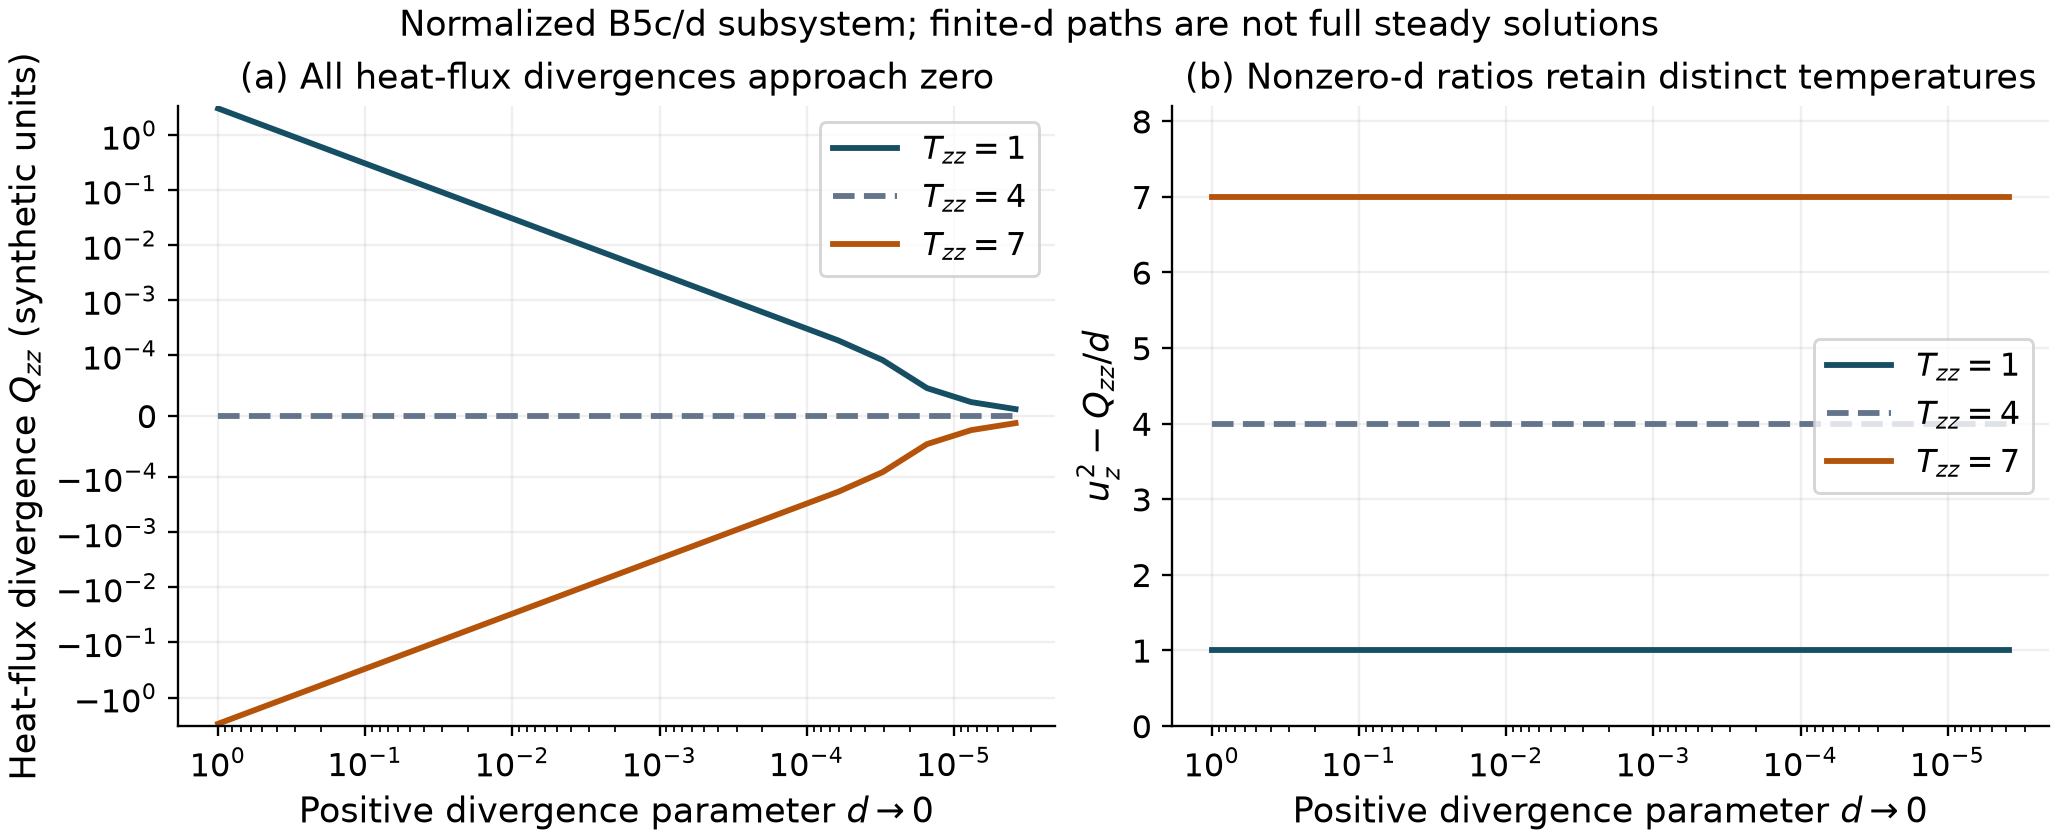
\includegraphics[keepaspectratio]{images/moment-compatibility.png}}

Figure 1. With \(n_i=m_i=e=1\), \(u=2\) and \(E_z=3\), each selected
positive \(T\) has \(S=3-2d\) and \(Q=(4-T)d\). All paths satisfy the
two normalized equations exactly. At \(d=0\), both numerator and divisor
of the rearranged expression vanish, and the temperature remains a
parameter. Finite-\(d\) paths fail the separately stated steady
uniform-density continuity assumption.
\end{minipage}

The source already recognizes a failure of its zero-heat-flux
approximation for the \(xx\) and \(yy\) moments on p.~21. That
acknowledgment should be retained. It does not remove the zero divisor
in the \(zz\) rearrangement. A related step, Eq. (B17), p.~22,
differentiates and extends a relation specialized to the X-point to the
sheet edge, where the preceding equations retain advection and magnetic
terms absent at the X-point. A neighborhood closure is needed to infer
that edge derivative and the range in (B18). Neither issue refutes the
temperatures plotted in Figs. 8-9. An electric field may contribute to
heating through particle orbits and phase-space mixing; a bulk
acceleration alone does not determine a central second moment.

\subsection{3. What a finite spatial mean
implies}\label{what-a-finite-spatial-mean-implies}

Appendix D, pp.~23-24, decomposes each quantity as
\(f=\langle f\rangle+\delta f\) and specifies two-dimensional spatial
Savitzky-Golay averaging. Its rationale separates small ion-acoustic
structures from larger reconnection structure. Fig. 10 labels
approximately \(0.22\,d_{e0}^{-1}\) as the reciprocal window length. The
exact point-count window, polynomial degree, two-dimensional
construction, edge mode and residual implementation were not obtained.
Window length alone does not specify a Savitzky-Golay frequency response
{[}3{]}.

For clarity, let a fixed normalized linear filter be

\[
(Gf)(\boldsymbol{x})=\sum_{\boldsymbol r}w_{\boldsymbol r}
f(\boldsymbol{x}+\boldsymbol r),\qquad
\sum_{\boldsymbol r}w_{\boldsymbol r}=1.\tag{6}
\]

Write \(N=Gn\), \(F=Gf\), and first interpret the fluctuation as the
pointwise field \(f'=f-Gf\). The exact covariance and filtered residual
product are distinct objects:

\[
C_{nf}=G(nf)-NF,\qquad R_{nf}=G(n'f').\tag{7}
\]

Expanding without Reynolds factorization gives

\[
\begin{aligned}
C_{nf}-R_{nf}={}&G[(Gn)(Gf)]-(Gn)(Gf)\\
&+G[(Gn)f']+G[n'(Gf)]\equiv K_{nf}.
\end{aligned}\tag{8}
\]

Normalization and linearity do not set these extra terms to zero. In
particular, \(Gf'=Gf-G^2f\) need not vanish. The distinction between
general spatial filters and Reynolds averages is established filtering
theory {[}4{]}, rather than a newly discovered failure of averaging. The
source-specific question is which of these operations its formulas and
postprocessing implement.

For species mass \(m\), signed charge \(q\), and \(U=G\boldsymbol u\),
source Eqs. (4.2) and (4.5) use residual-product expressions for drag
and the time-dependent fluctuation term. Under the pointwise
interpretation, an exact covariance formulation is instead

\[
\boldsymbol D_*=-\frac{C_{n\boldsymbol E}}{N},\qquad
\boldsymbol V_*=\frac{m}{qN}\,\partial_t C_{n\boldsymbol u}.\tag{9}
\]

Here the filter is fixed in time and \(N\) remains outside the time
derivative. Replacing \(C\) by \(R\) changes these terms by quantities
determined by Eq. (8); it is not justified by the field decomposition
alone. Conversely, the source's \(\boldsymbol T\) and \(\boldsymbol I\)
already retain full products:

\[
\begin{aligned}
\boldsymbol T&=-\frac{G[n(\boldsymbol u\times\boldsymbol B)]}{Nc}
+\frac{(G\boldsymbol u)\times(G\boldsymbol B)}c,\\
\boldsymbol I&=\frac{m}{qN}\left\{
G[\nabla\boldsymbol{\cdot}(n\boldsymbol u\boldsymbol u)]
-\nabla\boldsymbol{\cdot}(NUU)\right\}.
\end{aligned}\tag{10}
\]

They are positive controls for this particular algebraic issue.
Derivative commutation is a separate question: a constant interior
convolution commutes with the corresponding translation-invariant
derivative, while a position-dependent boundary rule need not. An
illustrative edge commutator does not establish the source's unspecified
edge treatment is wrong.

\subsection{4. An exact counterexample and an exact
alternative}\label{an-exact-counterexample-and-an-exact-alternative}

The five-point, degree-two Savitzky-Golay weights {[}3{]} are
\((-3,12,17,12,-3)/35\) at offsets \(r=-2,-1,0,1,2\). This kernel
reproduces quadratics. Set \(n(x)=2+x^2\) and \(E(x)=x^2\). Then
\(n'=E'=0\) everywhere for the infinite polynomial fields, so
\(R_{nE}=0\). At \(x=0\), however,

\[
N=2,\quad GE=0,\quad C_{nE}=-\frac{72}{35},
\quad D_*=\frac{36}{35},\quad D_{\rm residual}=0.\tag{11}
\]

The nonzero value comes from the degree-four product, which the
degree-two kernel does not reproduce. Negative Savitzky-Golay weights
allow a negative weighted covariance; this is not a negative
probabilistic variance or negative physical density. Both the density
and its filtered central value are positive. A separable two-dimensional
filter acting on fields independent of \(y\) gives the same example, so
the algebra is not rescued merely by specifying two dimensions.

A weaker density variation, \(n=2+x^2/100\), yields \(C_{nE}=-18/875\)
and \(D_*=9/875\). It can be embedded in an exact static primitive force
balance with positive pressure on the stencil neighborhood: take
\(q=1\), \(\boldsymbol u=\boldsymbol B=0\) and
\(P(x)=100+(2/3)x^3+x^5/500\), so \(\partial_xP=nE\). Filtering that
balance requires the full product \(G(nE)\). This is a deliberately
constructed moment-level counterexample, not a proposed reconnection
equilibrium or a replacement for any source field.

There is an essential counterargument to a source-code error allegation.
One can instead define a window-centered residual,

\[
\delta_{\boldsymbol x}f(\boldsymbol r)
=f(\boldsymbol x+\boldsymbol r)-(Gf)(\boldsymbol x).\tag{12}
\]

The same center mean is then subtracted at every sample in that
evaluation window. Direct expansion and normalization give

\[
\sum_{\boldsymbol r}w_{\boldsymbol r}
\delta_{\boldsymbol x}n(\boldsymbol r)
\delta_{\boldsymbol x}f(\boldsymbol r)
=G(nf)(\boldsymbol x)-(Gn)(\boldsymbol x)(Gf)(\boldsymbol x).
\tag{13}
\]

This is exact even for signed weights. It reproduces the nonzero
covariance in Eq. (11), while the pointwise residual field gives zero.
If the source implementation uses Eq. (12), its residual products can
already be the correct covariances. The available definition and absent
implementation do not decide between these conventions. Thus the
defensible source finding is an operator-definition and reproduction
gap, not a demonstrated error in Fig. 10 amplitudes.

\begin{minipage}{\linewidth}
\pandocbounded{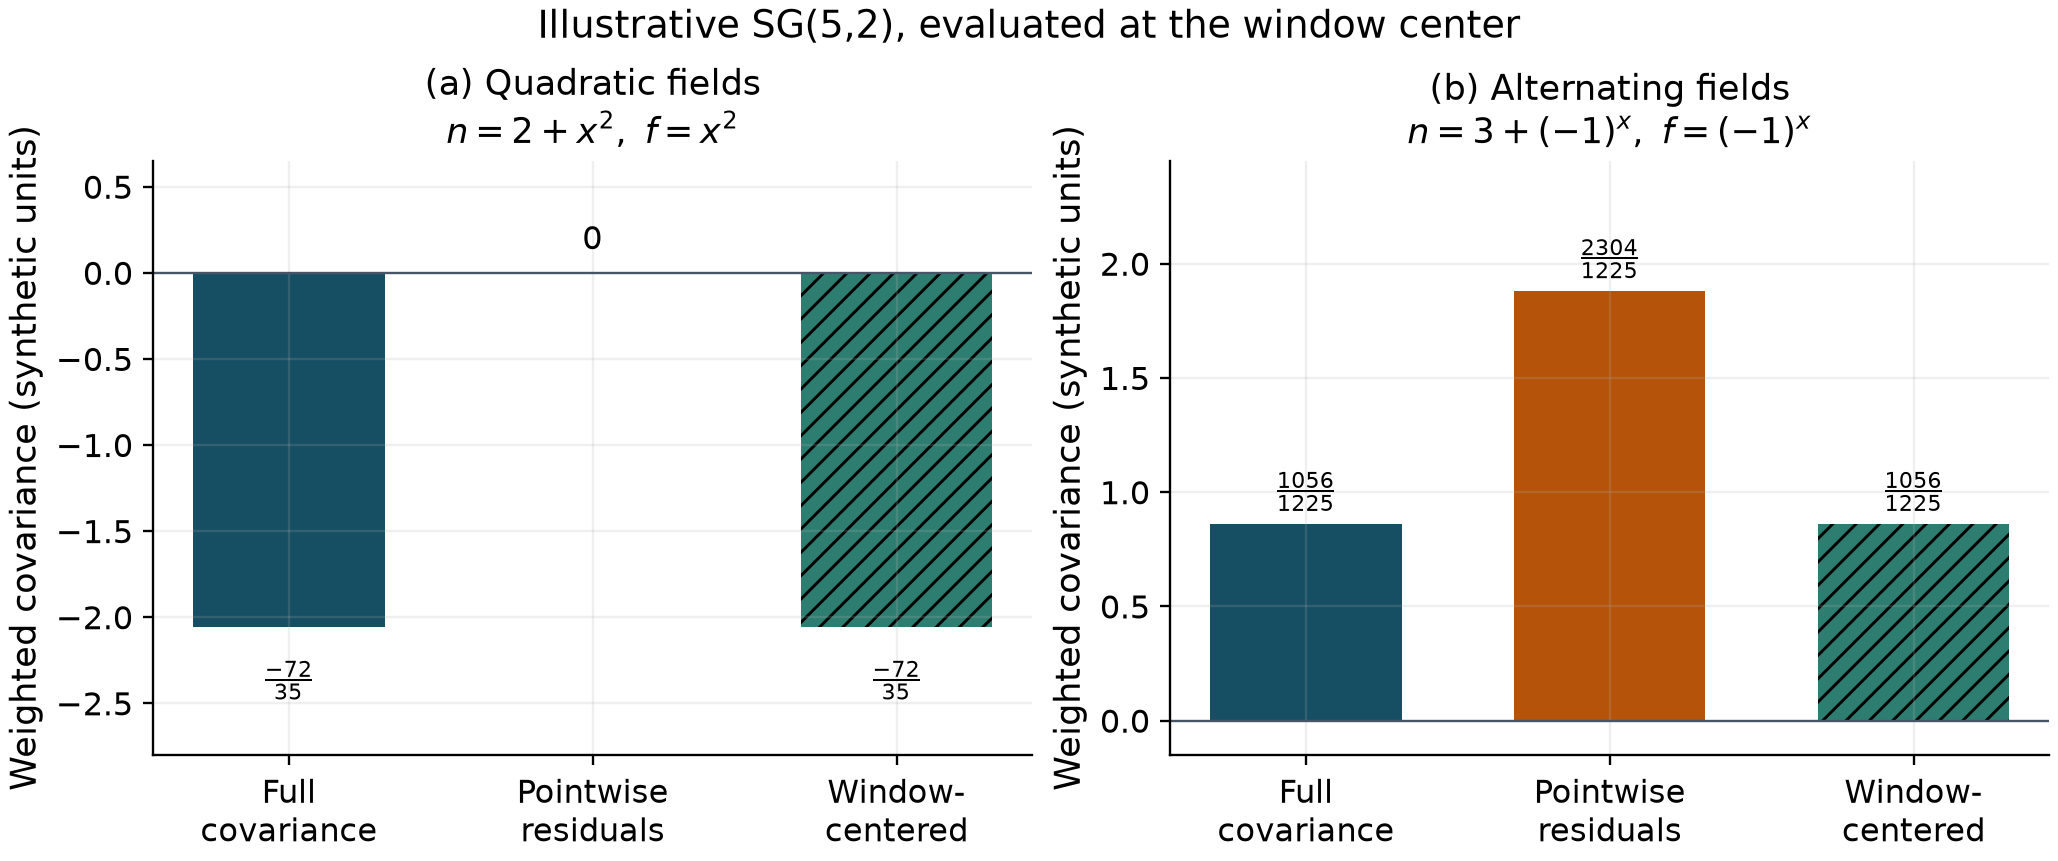
\includegraphics[keepaspectratio]{images/filter-covariance.png}}

Figure 2. Two original dimensionless examples use a five-point,
degree-two kernel. The polynomial case and an alternating-field case
distinguish full covariance from the filtered pointwise residual
product. The window-centered calculation agrees exactly with full
covariance in both. Neither example reconstructs the original filter,
density, electric field or plotted diagnostic.
\end{minipage}

The appropriate numerical repair, if needed, is to define the filter and
residual evaluation explicitly, compare the full covariance with the
implemented fluctuation product, and close the filtered momentum budget
using the same discrete derivatives. Without the original arrays, the
magnitude, sign and dynamical importance of any omitted term remain
unknown. A local force fluctuation also is not by itself a global
reconnection-rate or irreversible-heating measurement; the source
separately presents direct rate and temperature histories.

\subsection{5. Verification and retained
controls}\label{verification-and-retained-controls}

Original calculations {[}5{]} construct four synthetic centered
Savitzky-Golay kernels using exact rational least squares: window/degree
pairs \((5,2)\), \((7,3)\), \((9,2)\) and \((5,4)\). They check
polynomial reproduction, covariance decomposition and the exact
window-centered alternative in 20 cases. Forty time-dependent controls
check \(mC_{nf}/(qN)\) with both charge signs, including an
instantaneous force balance with
\(\boldsymbol u=\boldsymbol E=\boldsymbol B=0\),
\(\partial_t\boldsymbol u=f\) and \(\nabla\boldsymbol{\cdot}P=-mnf\).
The corresponding primitive momentum equation is satisfied at that
instant; no full kinetic evolution is asserted. Constants, the
degree-four identity kernel, a true broadcast ensemble mean, and the
source's full-product terms are retained controls.

The moment producer checks 273 exact states: seven positive selected
temperatures, each with \(d=\pm2^{-k}\) for \(k=0,\ldots,18\) and
\(d=0\). All satisfy the literal normalized (B5c)-(B5d) subsystem. The
266 nonzero-divergence states recover their selected temperature only
when division is legitimate, and all seven zero-divergence cases mark
Eq. (2) undefined. The \(T=4\) family is the zero-heat-flux,
nonzero-divisor positive control. Continuity violations at every
finite-\(d\) point are explicitly reported, rather than presented as
physical steady states.

Separate independent programs do not import the producer. One checks
filter identities, signed-charge time-dependent terms, derivative
commutation and the window-centered alternative using exact fractions.
Another verifies Maxwellian response identities, Harris/grid
normalization, homogeneous Doppler shifts and exact finite-mass marginal
thresholds, as well as two normalized moment witnesses. For mass ratio
100, its cold-ion threshold controls give \(U_d/c_s\simeq0.681520\) and
\(1.354021\), consistent with the source's stated 0.68 and 1.36 under
the declared local normalization. The Maxwellian susceptibility and the
final uniform nonrelativistic Doppler transformation pass; no
dispersion-calculation error is asserted from these controls.

An initially considered Appendix E mass-factor criticism is withdrawn.
Inverting its scale inequality for the existence of \emph{some} scale
below \(d_i\) differs from requiring the condition at \emph{every} scale
above \(d_e\). The latter uses \(d_e/d_i=\sqrt{m_e/m_i}\) and recovers
the printed mass factor in (E3). Its wording admits that universal
interpretation. Neither that candidate, a typical wavelength/FWHM
comparison, nor acknowledged mildly relativistic velocities establishes
an error in the PIC data. The source's explicit finite-mass-ratio and
three-dimensional caveats remain relevant.

The plotting producer was run under CPython 3.12.14, NumPy 2.3.5 and
Matplotlib 3.11.2; its algebra uses exact fractions, with floating point
restricted to plotting. Independent filter checks use the standard
library under CPython 3.13.7. Independent response/marginal checks use
CPython 3.13.7, NumPy 2.2.1 and SciPy 1.17.1. Actual environments and
original receipts are retained separately. Equality in these controls is
internal algebraic and computational evidence, not independent human
peer review or guaranteed bitwise portability across environments.

\subsection{6. Consequences and limits}\label{consequences-and-limits}

The temperature conclusion supported here is precise: under the stated
exact steady continuity assumptions, the divisor in (B6c) vanishes, and
its zero-heat-flux use does not determine (B10b). A consistent
approximate treatment must supply the missing relative order or a
different closure. This does not establish that the measured
out-of-plane temperature is incorrect, that the entire hierarchy has an
alternative steady solution, or that electric fields cannot participate
in heating.

For the anomalous terms, full covariances supply an exact operator
formulation, but the window-centered interpretation already yields them.
The source's actual code, fields and filtered budgets would be needed to
decide whether any numerical correction is required. No revised
anomalous amplitude, reconnection rate, physical mass-ratio simulation,
entropy-production result or complete kinetic reproduction is supplied.
The final edition's observed instability, measured temperature histories
and reported rate comparison remain separate evidence.

A focused revision could remove the zero-divisor inference, state the
assumptions needed for any replacement temperature estimate, and
document the exact filter kernel and residual convention with an
explicit budget-closure check. These steps make the analytical
interpretation reproducible while preserving conclusions that the
present audit has not tested.

\textbf{Code and data availability.} Original code, rational outputs,
two original figures, source-edition provenance and portable independent
checks accompany this study {[}5{]}. The verified software archive is
\url{https://doi.org/10.5281/zenodo.23782239} , direct record
\url{https://zenodo.org/records/23782239} , frozen at computational
commit \nolinkurl{36b1c070e029fd7e3c05e96af3b93172444bfee2} in
\url{https://github.com/Teylersf/ion-acoustic-moment-filter-audit} . All
three programs passed from a clean 42-file exported tree without
changing any archived file bytes. The anonymous archive download matches
that snapshot: 363,538 bytes, SHA-256
\nolinkurl{33d3f51c355896403154b1be4f4e13a2a652f69e80628ac9c8512abc97abd7b3}.
The DOI resolver and primary DataCite registry were checked on 29
October 2026; its state is \nolinkurl{findable}. The archive records actual
environments and distinguishes normalized subsystem tests from
unavailable original simulation data. Source PDFs and original figure
files are not presented as this author's work.

\textbf{Funding and disclosures.} Taylor Kalin self-funds this study. No
outside funding or competing interests have been reported. AI tools
assisted with retrieval, derivation, programming, adversarial checks and
drafting. These checks are not independent human peer review. The source
authors and institutions have not endorsed this comment. Original code
is MIT licensed; original audit text and figures are CC BY 4.0.
Attributed third-party material retains its rights.

\clearpage
\begingroup\small\raggedright
\subsection{References}\label{references}

{[}1{]} D. Li, Z. Liu and N. F. Loureiro, \emph{Role of ion acoustic
instability in magnetic reconnection}, Journal of Plasma Physics
\textbf{92}(1), E20 (2026).
\url{https://doi.org/10.1017/S002237782510113X} . Version of record,
published online 27 February 2026.

{[}2{]} D. Li, Z. Liu and N. F. Loureiro, \emph{Role of ion acoustic
instability in magnetic reconnection}, arXiv:2505.08983v1 (13 May 2025).
\url{https://arxiv.org/abs/2505.08983v1} ;
\url{https://arxiv.org/pdf/2505.08983v1} . Earlier edition, read
separately from {[}1{]}.

{[}3{]} A. Savitzky and M. J. E. Golay, \emph{Smoothing and
Differentiation of Data by Simplified Least Squares Procedures},
Analytical Chemistry \textbf{36}(8), 1627-1639 (1964).
\url{https://doi.org/10.1021/ac60214a047} . Bibliographic metadata
verified in the primary Crossref record; complete prior-paper reading is
not claimed.

{[}4{]} M. Germano, \emph{Turbulence: the filtering approach}, Journal
of Fluid Mechanics \textbf{238}, 325-336 (1992).
\url{https://doi.org/10.1017/S0022112092001733} . The public publisher
abstract explicitly distinguishes general filters from Reynolds
averaging and discusses generalized central moments; that content check
is limited to the abstract.

{[}5{]} T. Kalin, \emph{Computational evidence for Continuity and
spatial averaging in ion-acoustic reconnection diagnostics}, software
version 1.0.0, Zenodo (2026).
\url{https://doi.org/10.5281/zenodo.23782239} ;
\url{https://zenodo.org/records/23782239} . Primary DataCite
registration:
\url{https://api.datacite.org/dois/10.5281/zenodo.23782239} .
Computational snapshot
\nolinkurl{36b1c070e029fd7e3c05e96af3b93172444bfee2}.

\endgroup
